\documentclass[10pt]{report}
\usepackage[utf8]{inputenc}
\usepackage{amsfonts}
\usepackage{amsmath}
\usepackage{amssymb}
\usepackage{commath}
\usepackage[ngerman]{babel}
\usepackage{enumitem}
\usepackage{booktabs}
\usepackage{longtable}
\usepackage{relsize}
\usepackage{pgfplots}
\usepackage{csvsimple}
\usepackage{pgfplotstable}
\usepackage{siunitx}
\usepackage{fancyhdr}
\usepackage{color}
\usepackage{float}
\usepackage{listings}

\definecolor{mygreen}{RGB}{28,172,0} % color values Red, Green, Blue
\definecolor{mylilas}{RGB}{170,55,241}


\lstset{language=Matlab,%
    %basicstyle=\color{red},
    breaklines=true,%
    morekeywords={matlab2tikz},
    keywordstyle=\color{blue},%
    morekeywords=[2]{1}, keywordstyle=[2]{\color{black}},
    identifierstyle=\color{black},%
    stringstyle=\color{mylilas},
    commentstyle=\color{mygreen},%
    showstringspaces=false,%without this there will be a symbol in the places where there is a space
    %numbers=left,%
    %numberstyle={\tiny \color{black}},% size of the numbers
    %numbersep=9pt, % this defines how far the numbers are from the text
    emph=[1]{for,end,break},emphstyle=[1]\color{red}, %some words to emphasise
    %emph=[2]{word1,word2}, emphstyle=[2]{style},
}

\setlength\parindent{0pt}

\setcounter{chapter}{4}
\setcounter{secnumdepth}{3}


\pagestyle{fancy}
\fancyhf{}
\lhead{GPET Versuch 3}
\rhead{Tim Luchterhand, Paul Nykiel}
\cfoot{\thepage}

\author{Tim Luchterhand, Paul Nykiel}
\title{GPET Versuch 3}

\begin{document}
        \maketitle

        \section{Messung harmonischer Signale}
        \subsection{Einstellung des Oszilloskops}
        \paragraph{Einführung}
        Melden Sie sich zunächst mit ihrem kiz-Account im webvpn an und starten sie die GUI.\@
        Verbinden Sie anschließend den Funktionsgenerator des Oszilloskops über ein BNC Kabel
        mit Kanal 1 des Oszilloskops. Stellen Sie in der GUI für den Funktionsgenerator ein Sinussignal der Frequenz 697 Hz und der Amplitude 1 V ein. Verwenden Sie für die folgenden
        Messungen lediglich die im Oszilloskop integrierten Messfunktionen.

        \subsubsection{Überprüfen der Funktion}
        \paragraph{Aufgabe}
        Überprüfen Sie, ob die von Ihnen gesetzte Einstellungen für den Funktionsgenerator
        der auf dem Schirm des Oszilloskops dargestellten Funktion entsprechen.

        \paragraph{Protokoll}
        \begin{center}
            \begin{figure}[H]
                %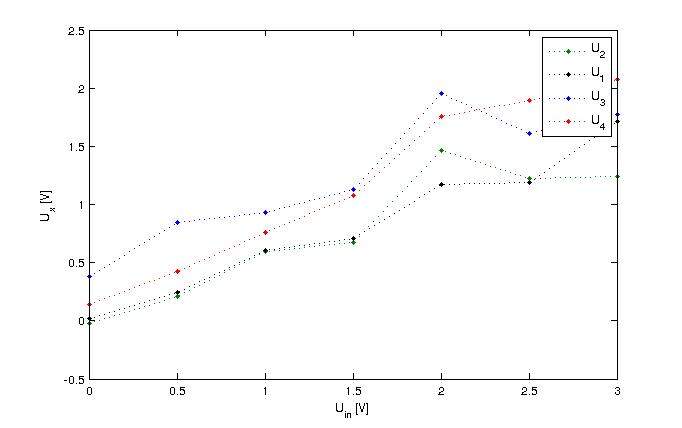
\includegraphics[width=\textwidth]{KPVmess.jpg}
              \caption{Oszilloskop Screenshot}
            \end{figure}
            \begin{figure}[H]
                %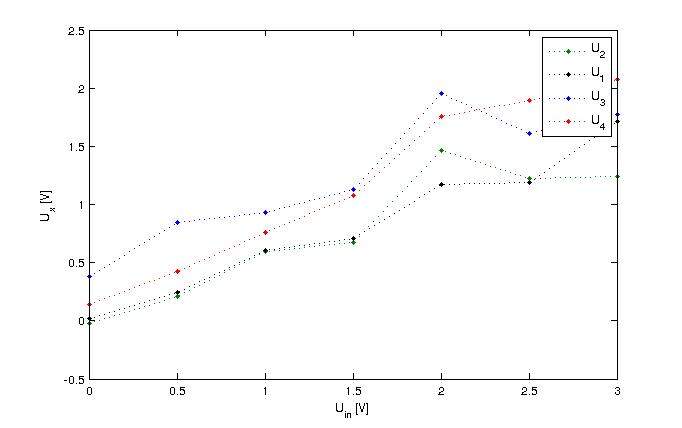
\includegraphics[width=\textwidth]{KPVmess.jpg}
              \caption{GUI Screenshot}
            \end{figure}
        \end{center}
        \subsubsection{Measure-Funktion}
        \paragraph{Aufgabe}
        Geben Sie die Peak-to-Peak Spannung, den Effektivwert, den Offset und die Frequenz
        des Signals an. Verwenden Sie dazu die \glqq{}Meas.\grqq-{}Funktion und die Cursor des
        Oszilloskops.
        \paragraph{Protokoll}
        \begin{center}
            \begin{figure}[H]
                %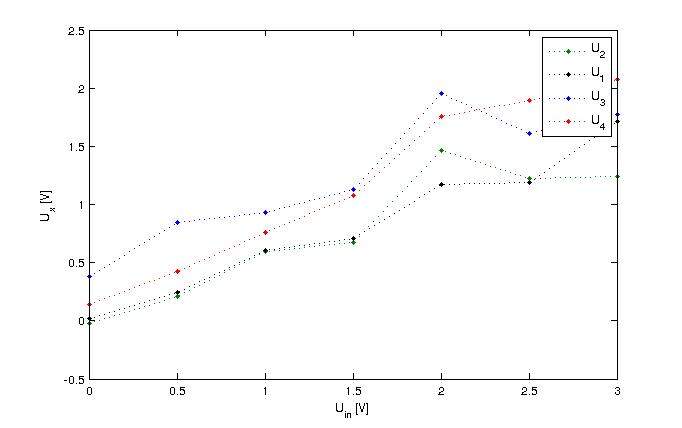
\includegraphics[width=\textwidth]{KPVmess.jpg}
              \caption{GUI Screenshot}
            \end{figure}
        \end{center}

        \subsubsection{Plot}
        \paragraph{Aufgabe}
        Stellen Sie die Skalierung der Anzeige über die GUI so ein, dass $5 - 8$ Perioden des
        Signals angezeigt werden und geben Sie die Amplitude des Signals an. Speichern
        Sie den Plot und fügen Sie ihn in das Protokoll ein.
        \paragraph{Protokoll}
        \begin{center}
            \begin{figure}[H]
                %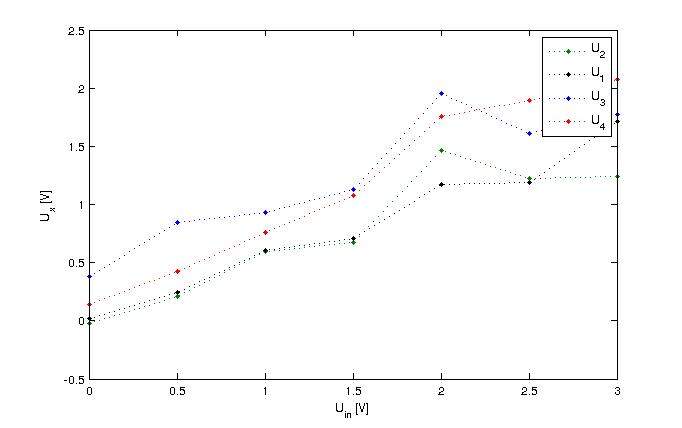
\includegraphics[width=\textwidth]{KPVmess.jpg}
              \caption{GUI Screenshot}
            \end{figure}
        \end{center}

        \subsection{Fourier-Transformation}
        \paragraph{Einführung}
        Das Oszilloskop verfügt intern über die Möglichkeit die Fourier Transformierte des dargestellten
        Zeitsignals zu berechnen. Diese soll im Folgenden verwendet werden.
        Die Auswahl der FFT-Funktion am Oszilloskop erfolgt über
        \glqq{}Math\grqq{} $\rightarrow$ \glqq{}Operator\grqq{} $\rightarrow$ \glqq{}FFT\grqq{}.
        Anschließend mussen Spanne und Mittenfrequenz entsprechend des darzustellenden Frequenzbereichs gewählt werden.
        Unter \glqq{} Mehr FFT\grqq{} lassen sich weitere Einstellungen
        zur FFT vornehmen: die Fensterfunktion und die vertikale Einheit.
        Mit Hilfe einer Fensterfunktion lässt sich der sogenannte \glqq{}Leakage effect\grqq{} vermindern.
        Dieser tritt in der in der digitalen Signalverarbeitung auf, wenn Blocklängen des zu verarbeitenden
        Signals endlich sind. Hier soll das \glqq{}Hanning-Fenster\grqq{} als Voreinstellung beibehalten
        werden.
        Für die vertikale Skalierung gibt es die beiden Möglichkeiten \glqq{}Decibel\grqq{} und
        \glqq{}$\text{V}_{\text{RMS}}$\grqq{}.
        In der Einstellung \glqq{}
        Decibel\grqq{} wird die vertikale Achse logarithmisch aufgetragen, in der
        Einstellung \glqq{}$\text{V}_{\text{RMS}}$\grqq{} linear. Die Rauschleistung ist in diesem Versuch im Allgemeinen sehr
        viel kleiner als die Signalleistung. Deshalb ist in der linearen Auftragung mit dem bloßen
        Auge kein Rauschen sichtbar. Aufgrund dessen wählt man für Spektren in der Regel auch
        die logarithmische Darstellung, welche im Folgenden auch immer gewählt werden sollte.
        Die vertikale Einstellung lässt sich nicht uber die GUI ändern, diese muss immer händisch
        am Oszilloskop eingestellt werden.
        \subsubsection{FFT mit dem Oszilloskop}
        \paragraph{Aufgabe}
        Wenden Sie die im Oszilloskop integrierte FFT-Funktion auf das Zeitsignal aus
        Teil 1 an um das Spektrum zu bestimmen, plotten sie dieses und geben Sie die
        gemessene Frequenz an. Sie können die Einstellungen zur FFT entweder direkt
        am Oszilloskop oder über die GUI vornehmen. Beachten Sie dabei, dass sie den
        dargestellten Frequenzbereich dem Signal entsprechend sinnvoll wählen. Erfassen
        Sie das Spektrum uber die GUI und fügen Sie es in das Protokoll ein.
        \paragraph{Protokoll}
        \begin{center}
            \begin{figure}[H]
                %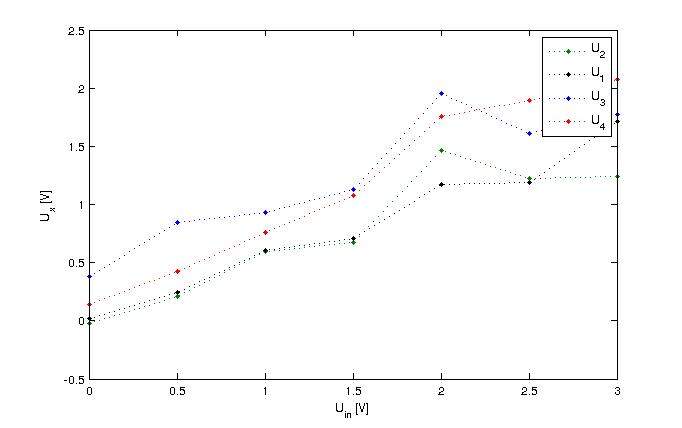
\includegraphics[width=\textwidth]{KPVmess.jpg}
              \caption{GUI Screenshot}
            \end{figure}
        \end{center}
        \subsubsection{Akustische Ausgabe}
        \paragraph{Aufgabe}
        Das Signal lässt sich am PC akustisch ausgeben. Dazu muss das Zeitsignal mit
        der GUI aufgenommen werden. Wählen Sie dazu im Bereich Measurements Type
        \glqq{}Wave\grqq{} und den entsprechenden Kanal. Über den Button \glqq{}Start\grqq{} wird die Messung
        gestartet. Anschließend kann das Signal in der GUI im Bereich \glqq{}Data\grqq{} ausgewählt
        werden und durch drücken des Button \glqq{}Sound\grqq{} abgespielt werden. Achten Sie darauf,
        dass die Lautstärke in Windows nicht zu leise oder ganz abgeschaltet ist. Hören
        Sie sich das Signal an und beschreiben Sie Ihren Höreindruck.
        \paragraph{Protokoll}
        \begin{center}
            \begin{figure}[H]
                %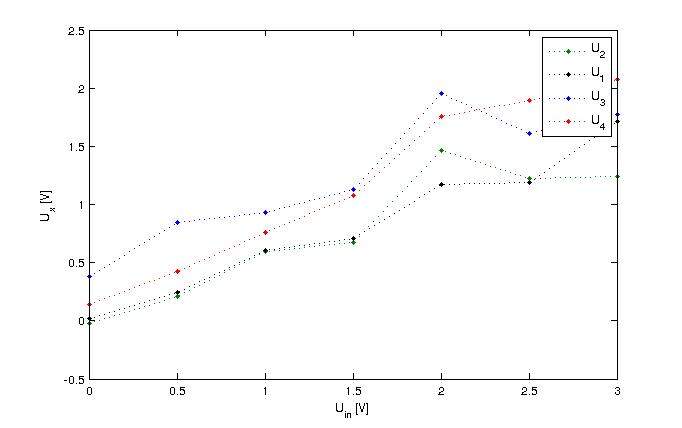
\includegraphics[width=\textwidth]{KPVmess.jpg}
              \caption{GUI Screenshot}
            \end{figure}
        \end{center}

        \subsection{FFT vs. Gehör}
        \paragraph{Aufgabe}
        Stellen Sie am Funktionsgenerator des Oszilloskops unter Verwendung der GUI ein Sinussignal
        der Frequenz $1477\si{\hertz}$ und der Amplitude $1\si{\volt}$ und einem Offset von $100\si{m\volt}$
        ein.
        \paragraph{Protokoll}
        \begin{center}
            \begin{figure}[H]
                %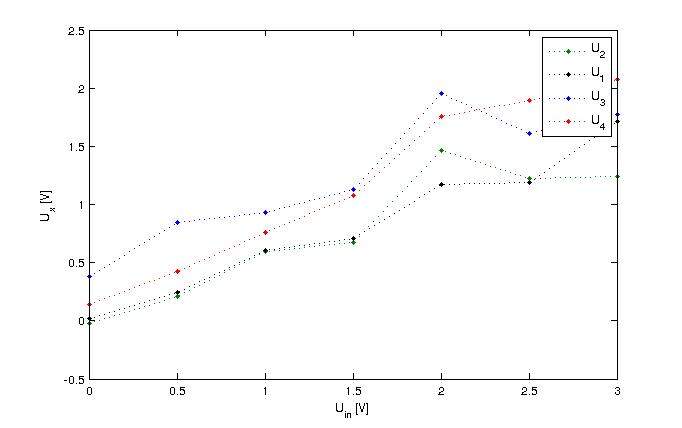
\includegraphics[width=\textwidth]{KPVmess.jpg}
              \caption{GUI Screenshot}
            \end{figure}
        \end{center}

        \subsubsection{Plot}
        \paragraph{Aufgabe}
        Plotten Sie das Signal in Zeit- und Frequenzbereich und geben Sie dabei die Amplitude
        und den Offset bzw.\ die gemessene Frequenz an. Wählen Sie den dargestellten
        Zeitabschnitt so, dass der Signalverlauf erkannt werden kann. Weshalb spielt der
        Offset im Frequenzbereich keine Rolle?
        \paragraph{Protokoll}
        \begin{center}
            \begin{figure}[H]
                %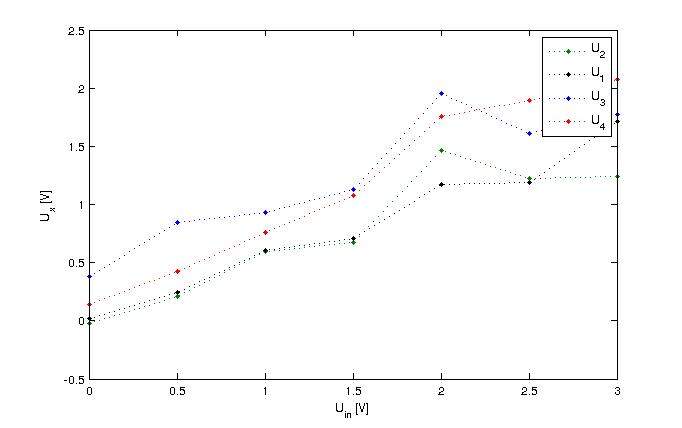
\includegraphics[width=\textwidth]{KPVmess.jpg}
              \caption{GUI Screenshot}
            \end{figure}
        \end{center}

        \subsubsection{Höreindruck}
        \paragraph{Aufgabe}
        Hören Sie sich das Signal an und vergleichen Sie den Höreindruck mit dem zuvor
        abgespielten Signal.
        \paragraph{Protokoll}
        \begin{center}
            \begin{figure}[H]
                %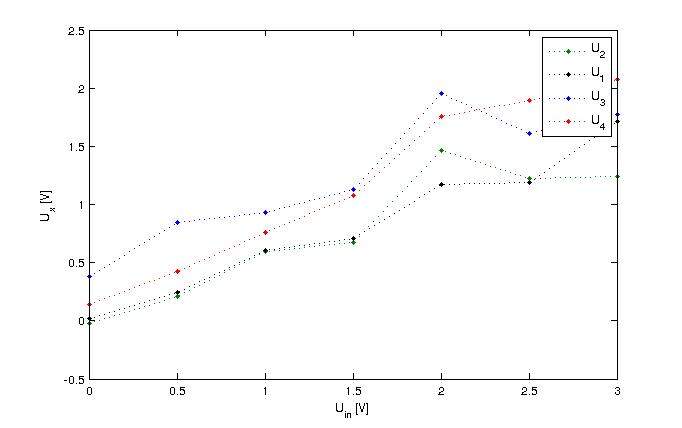
\includegraphics[width=\textwidth]{KPVmess.jpg}
              \caption{GUI Screenshot}
            \end{figure}
        \end{center}

        \subsubsection{Höreindruck bei kleinen Frequenz-Differenzen}
        \paragraph{Aufgabe}
        Stellen Sie nun ein Signal der Frequenz $1480\si{\hertz}$ und der Amplitude $1\si{\volt}$ am Funktionsgenerator
        ein und hören Sie sich auch dieses Signal an. Können die beiden
        Signale mit Frequenzen von $1477\si{\hertz}$ und $1480\si{\hertz}$ akustisch voneinander unterschieden
        werden? Wenn nicht, weshalb ist dies nicht möglich?
        \paragraph{Protokoll}
        \begin{center}
            \begin{figure}[H]
                %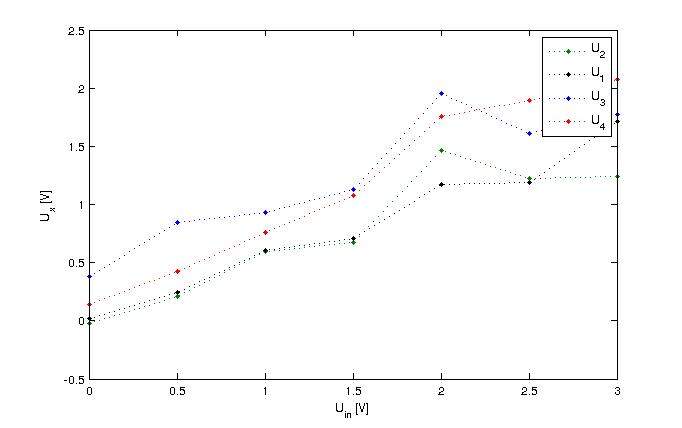
\includegraphics[width=\textwidth]{KPVmess.jpg}
              \caption{GUI Screenshot}
            \end{figure}
        \end{center}

        \subsubsection{Auflösung}
        \paragraph{Auflösung}
        Wie groß muss dass Messintervall gewählt werden, damit diese beiden Signale
        mittels FFT unterschieden werden können? Wie vielen Perioden des Signals mit
        $1480\si{\hertz}$ entspricht dies?
        \paragraph{Protokoll}
        \begin{center}
            \begin{figure}[H]
                %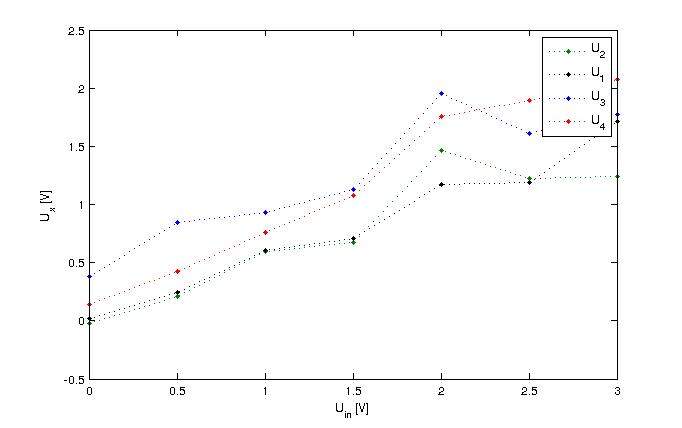
\includegraphics[width=\textwidth]{KPVmess.jpg}
              \caption{GUI Screenshot}
            \end{figure}
        \end{center}


        \section{Messung periodischer Signale}
        \paragraph{Einführung}
        Verbinden Sie den Eingang des externen Trigges am Oszilloskop (auf der Rückseite) und
        den \glqq{}TTL/CMOS OUTPUT\grqq{} des externen Funktionsgenerators mit einem BNC Kabel.
        Bei einigen Funktionsgeneratoren muss der \glqq{}SYNC Out\grqq{} gewählt werden. Stellen Sie
        anschließend den Trigger des Oszilloskops auf \glqq{}extern\grqq{} ein. Das Oszilloskop wird nun auf
        das Signal des externen Frequenzgenerators getriggert.
        Im Folgenden werden ein Signal des externen und ein Signal des internen Funktionsgenerators
        über ein T-Stück addiert und auf Kanal 1 geführt.
        Verbinden Sie dazu den Ausgang des externen Funktionsgenerators über die eine Seite
        des T-Stücks mit Kanal 1 des Oszilloskops. Stellen Sie nun ein Sinussignal der Frequenz
        697 Hz ein. VSS soll dabei etwa 2 V betragen. Überprüfen Sie die Amplitude des Signals
        auf dem Schirm des Oszilloskops.
        Stellen Sie am Funktionsgenerator des Oszilloskops ein Signal der Frequenz 1336 Hz,
        Amplitude 1 V und Offset 0 V ein. Addieren Sie die beiden Signale unter Verwendung des
        T-Stücks indem Sie das Ausgangssignal des Funktionsgenerators des Oszilloskops über
        ein BNC-Kabel auf das zweite Ende des T-Stücks geben.

        \subsubsection{Stehende Welle}
        \paragraph{Aufgabe}
        Wieso erhält man keine stehende Welle auf dem Schirm des Oszilloskops? Weshalb
        spielt das bei der Berechnung der FFT keine Rolle?
        \paragraph{Protokoll}


        \subsubsection{Plot}
        \paragraph{Aufgabe}
        Plotten Sie einen geeigneten Ausschnitt des Summensignals im Zeitbereich. Geben
        Sie den Minimal- und Maximalwert des Signals an.
        \paragraph{Protokoll}

        \subsubsection{Höreindruck}
        \paragraph{Aufgabe}
        Hören Sie sich einen geeigneten Zeitausschnitt des Summensignals mit Hilfe der
        \glqq{}Sound\grqq{}-Funktion an und beschreiben Sie den Höreindruck.
        \paragraph{Protokoll}

        \subsubsection{Frequenzbereich}
        \paragraph{Aufgabe}
        Transformieren Sie das Signal in den Frequenzbereich und plotten Sie es. Geben Sie
        die auftretenden Frequenzen an.
        \paragraph{Protokoll}

        \subsubsection{Bandbreite}
        \paragraph{Aufgabe}
        Geben Sie die Bandbreite sowie die obere und untere Grenzfrequenz des Signals an.
        \paragraph{Protokoll}

        \section{Mehrfrequenzwahlverfahren}
        \begin{center}
            \begin{figure}[H]
                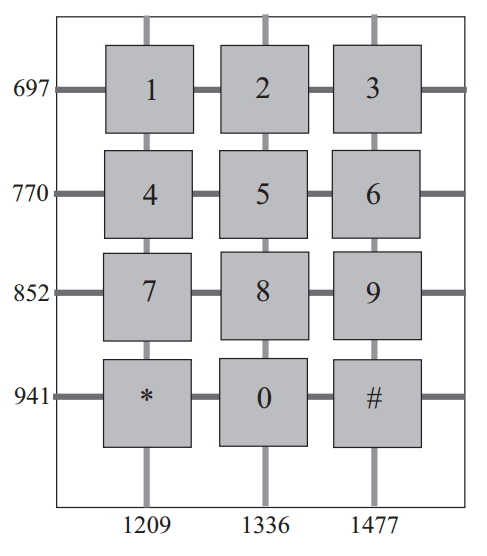
\includegraphics[width=\textwidth]{dtmf_pad.jpg}
                \caption{DTMF Tasten}
            \end{figure}
        \end{center}
        \subsection{DTMF-App}
        \paragraph{Aufgabe}
        Für diesen Versuchsteil benötigen Sie nun die zuvor auf Ihr Mobiltelefon geladene \glqq{}DTMF\grqq{} App.
        Verbinden Sie den Kopfhörerausgang Ihres Mobiltelefons mit einem 3.5 mm Klinke-Kabel
        über das Steckbrett mit Kanal 1 des Oszilloskops. Parallel dazu schalten Sie einen Kopfhörer.

        Schauen Sie sich die Frequenzen einzelner Töne mit der Fourier-Transformation auf dem
        Oszilloskop an. Beschreiben Sie Ihren Höreindruck sowie Ihre Beobachtungen auf dem
        Oszilloskop bei einer waagrechten, senkrechten und diagonalen Tastenfolge.
        \paragraph{Protokoll}

        \subsection{Matlab}
        \paragraph{Einführung}
        Im Folgenden sollen die zuvor durch die beiden Funktionsgeneratoren realisierten Oszillatoren
        in MATLAB umgesetzt werden. Dadurch sollen zunächst einige Töne, wie sie
        beim Mehrfrequezwahlverfahren verwendet werden synthetisiert und im abschließenden
        Versuchsteil eine \glqq{}gewählte\grqq{} Telefonnummer unter Verwendung der FFT analysiert werden.
        Oszilloskop, BNC Kabel und Frequenzgenerator werden in diesem Versuchsteil nicht
        mehr benötigt.
        Laden Sie sich das Archiv \texttt{DTMF\_Student.zip} von der Praktikumsseite herunter und
        entpacken Sie es. Wechseln Sie anschließend innerhalb von MATLAB in den Ordner mit
        den entpackten Dateien. Hier finden Sie folgenden MATLAB Files:
        \begin{itemize}
            \item \texttt{dial\_tones.m}

                Spielt die vom Benutzer gewählte Nummer ab und plottet die DTMF-Töne in Zeit-
                und Frequenzbereich. Zwischen den einzelnen Ziffern wird dabei eine Pause der
                Länge \texttt{pauslen} eingefügt.

            \item \texttt{dialed\_number.mat}

                MATLAB Stuct, mit der zu analysierenden Nummer. Zur Weiteren Verabeitung
                muss das Struct zunächst in MATLAB importiert werden. Dies kann über einen
                Rechtsklick auf das File ausgewählt werden.

            \item \texttt{dtmfcut.m}

                Wird verwendet um die gesendete Nummer in einzelne Zeitabschnitte zu zerlegen
                und die Fourier Transformierte über diese einzelnen Zeitabschnitte zu berechnen.
                Der Aufruf erfolgt automatisch innerhalb der Funktion \texttt{receive\_dial}.

            \item \texttt{fft\_dtmf.m}

                Diese Funktion enthält ein Codefragment das während dieses Praktikumsversuchs
                vervollständigt werden soll um die gespeicherte Telefonnummer in Zeit- und Fre-
                quenzbereich zu plotten und anhören zu können.

            \item \texttt{generate\_tones.m}

                Erzeugt die entsprechenden DTMF Töne, wenn eine Taste entsprechend der Tastenbelegung aus Abbildung 10 gewählt wird. Die Eingabe muss dabei nach der
                Eingabeaufforderung als String erfolgen. Diese Funktion enthält einige Lücken und muss während des Versuchs
                vervollständigt werden.

            \item \texttt{receive\_dial.m}

                Gibt die gewählte Telefonnummer zurück, indem das gewählte Signal mittels FFT
                analysiert wird. Zusätzlich wird jede einzelne erkannte Ziffer in Zeit und Frequenz-
                bereich geplottet.
        \end{itemize}

        \subsection{Sourcecode}
        \paragraph{Aufgabe}
        In der Datei \texttt{generate\_tones.m} fehlen einige Zeilen. Vervollständigen Sie den Code. Die
        Korrektheit des Codes kann durch Aufruf der Funktion \texttt{dial\_tones.m} überprüft werden.
        (Eingabe von \texttt{dial\_tones();} im Commandwindow und in der Eingabeaufforderung dann
        beispielsweise ’2’, achten sie auf die Hochkommata).
        \paragraph{Protokoll}
        \lstinputlisting[language=Matlab, firstline=10, lastline=19]{generate_tones_Student.m}

        \vspace{2cm}

        \lstinputlisting[language=Matlab, firstline=85, lastline=92]{generate_tones_Student.m}

        \subsection{FFT Tastentöne}
        \subsubsection{Plots des Mehrfrequenzverfahrens}
        \paragraph{Aufgabe}
        Verwenden Sie die Funktion \texttt{dial\_tones} um das Signal für die Taste
        \glqq{}1\grqq{} im Mehrfrequenzwahlverfahren
        zu erzeugen und hören Sie es sich an. Geben Sie die auftretenden
        Frequenzen an und fügen Sie die beiden Plots in das Protokoll ein. Skalieren
        Sie die Diagramme dafür sinnvoll.
        \paragraph{Protokoll}
        \begin{center}
            \begin{figure}[H]
                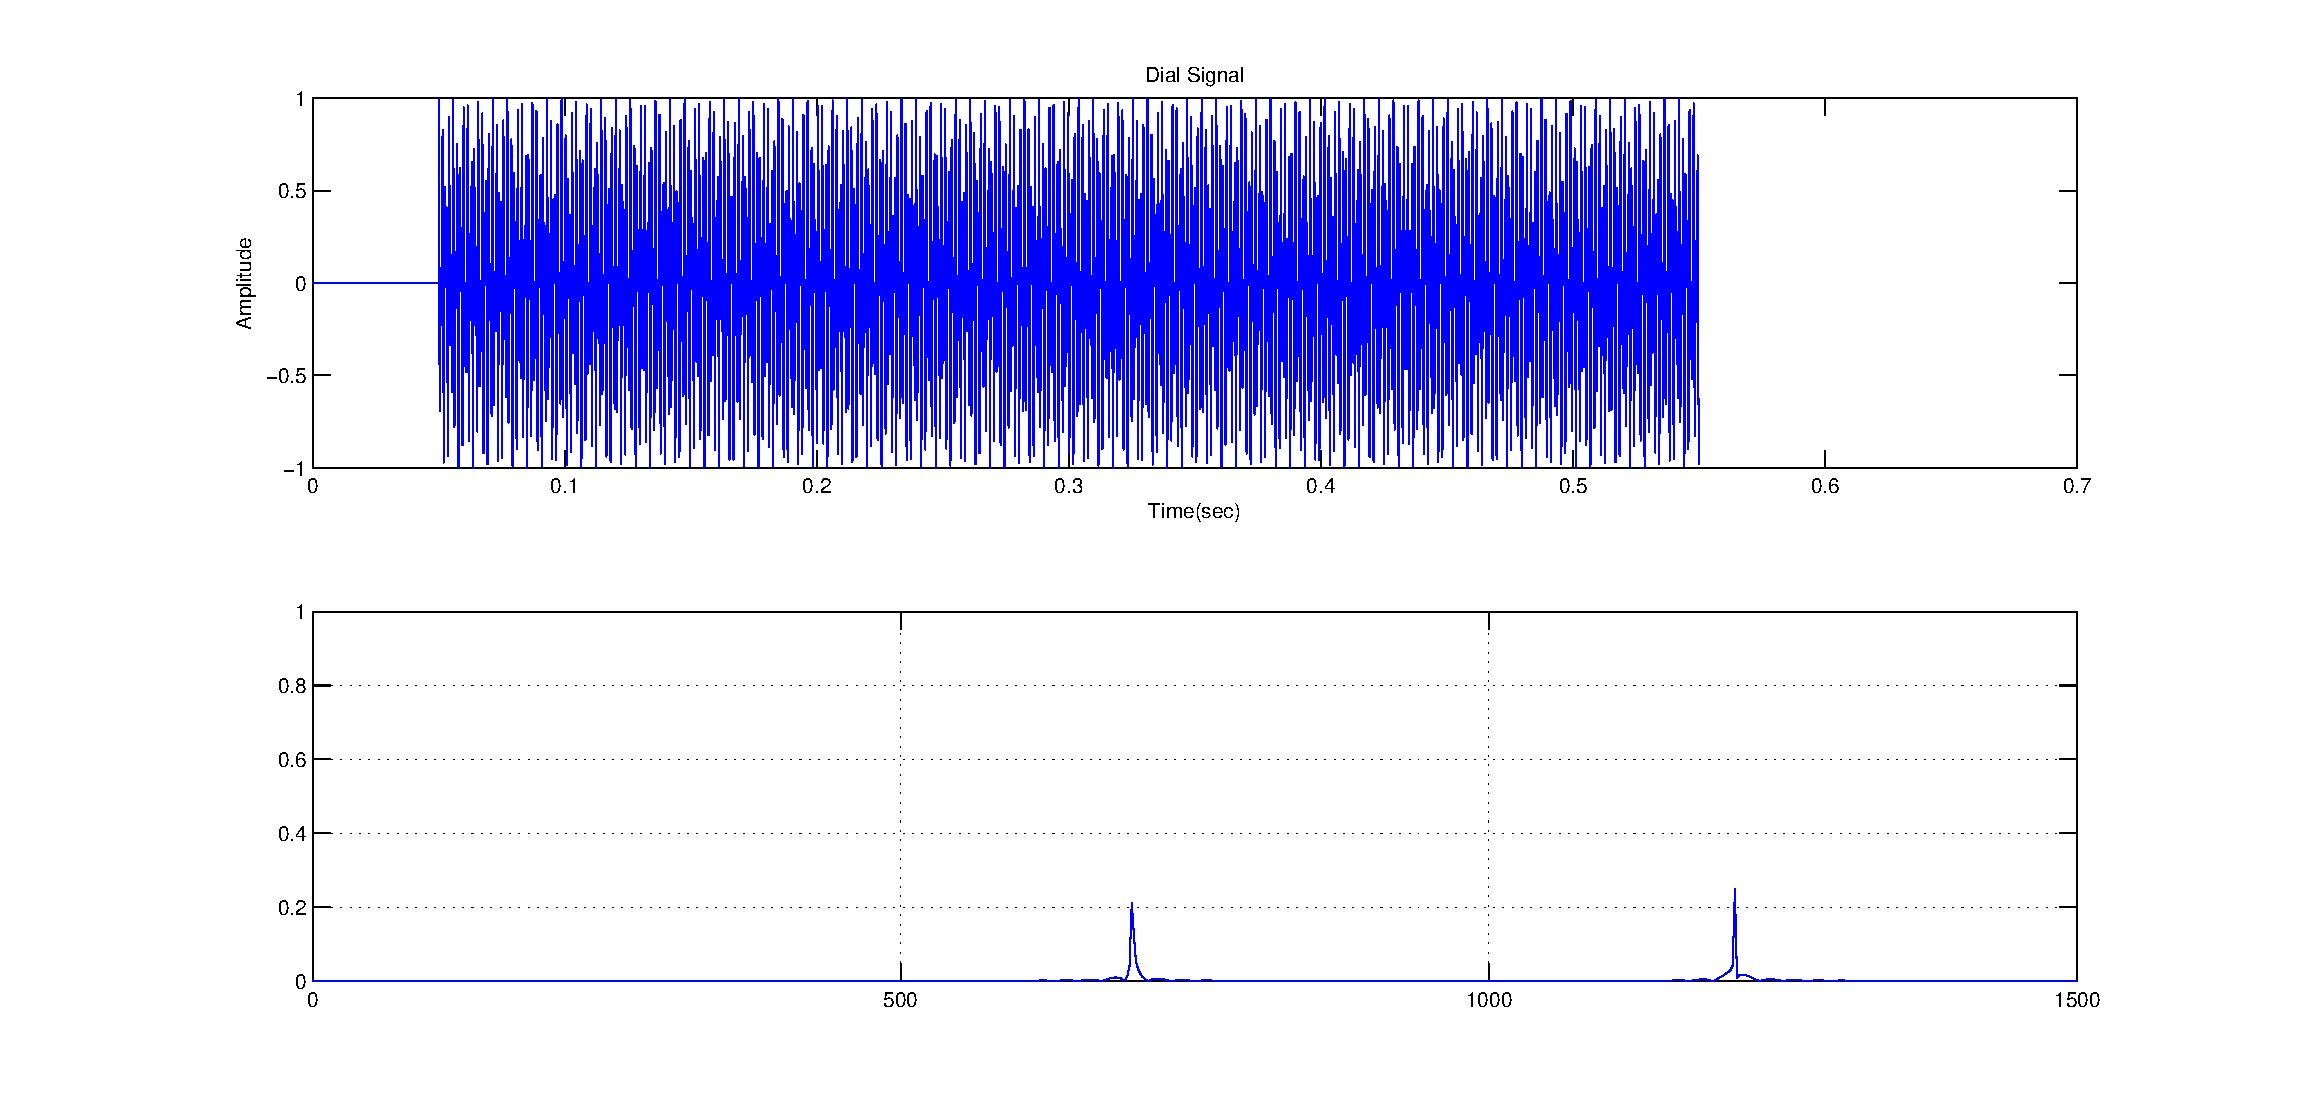
\includegraphics[width=\textwidth]{img4341}
              \caption{\texttt{dial\_tones} mit Eingabe \texttt{1}}
            \end{figure}
        \end{center}
        Auftretende Frequenzen:
        \begin{eqnarray*}
            f_{1_{fft}} &=& 696.38 \si{\hertz}\\
            f_{1_{soll}} &=& 697\si{\hertz}\\
            f_{2_{fft}} &=& 1209.12\si{\hertz}\\
            f_{2_{soll}} &=& 1209\si{\hertz}
        \end{eqnarray*}
        Die im Diagramm abgelesenen Frequenzen weichen nur sehr gering von den
        eingestellten Frequenzen ab. Die Frequenzen lassen sich immer noch eindeutig
        einer Ziffer zuordnen.

        Die geringe Abweichung ist der Umrechnung
        vom Frequenzbereich zum Bildbereich und wieder zurück geschuldet.

        \subsubsection{Tastentöne}
        \paragraph{Aufgabe}
        Hören Sie sich 2 weitere beliebige Tastentöne an und analysieren Sie die Signale im
        Frequenzbereich. Verwenden Sie dazu erneut die Funktion \texttt{dial\_tones} und wählen
        Sie jeweils nur eine Ziffer auf einmal.
        \paragraph{Protokoll}

        \begin{center}
            \begin{figure}[H]
                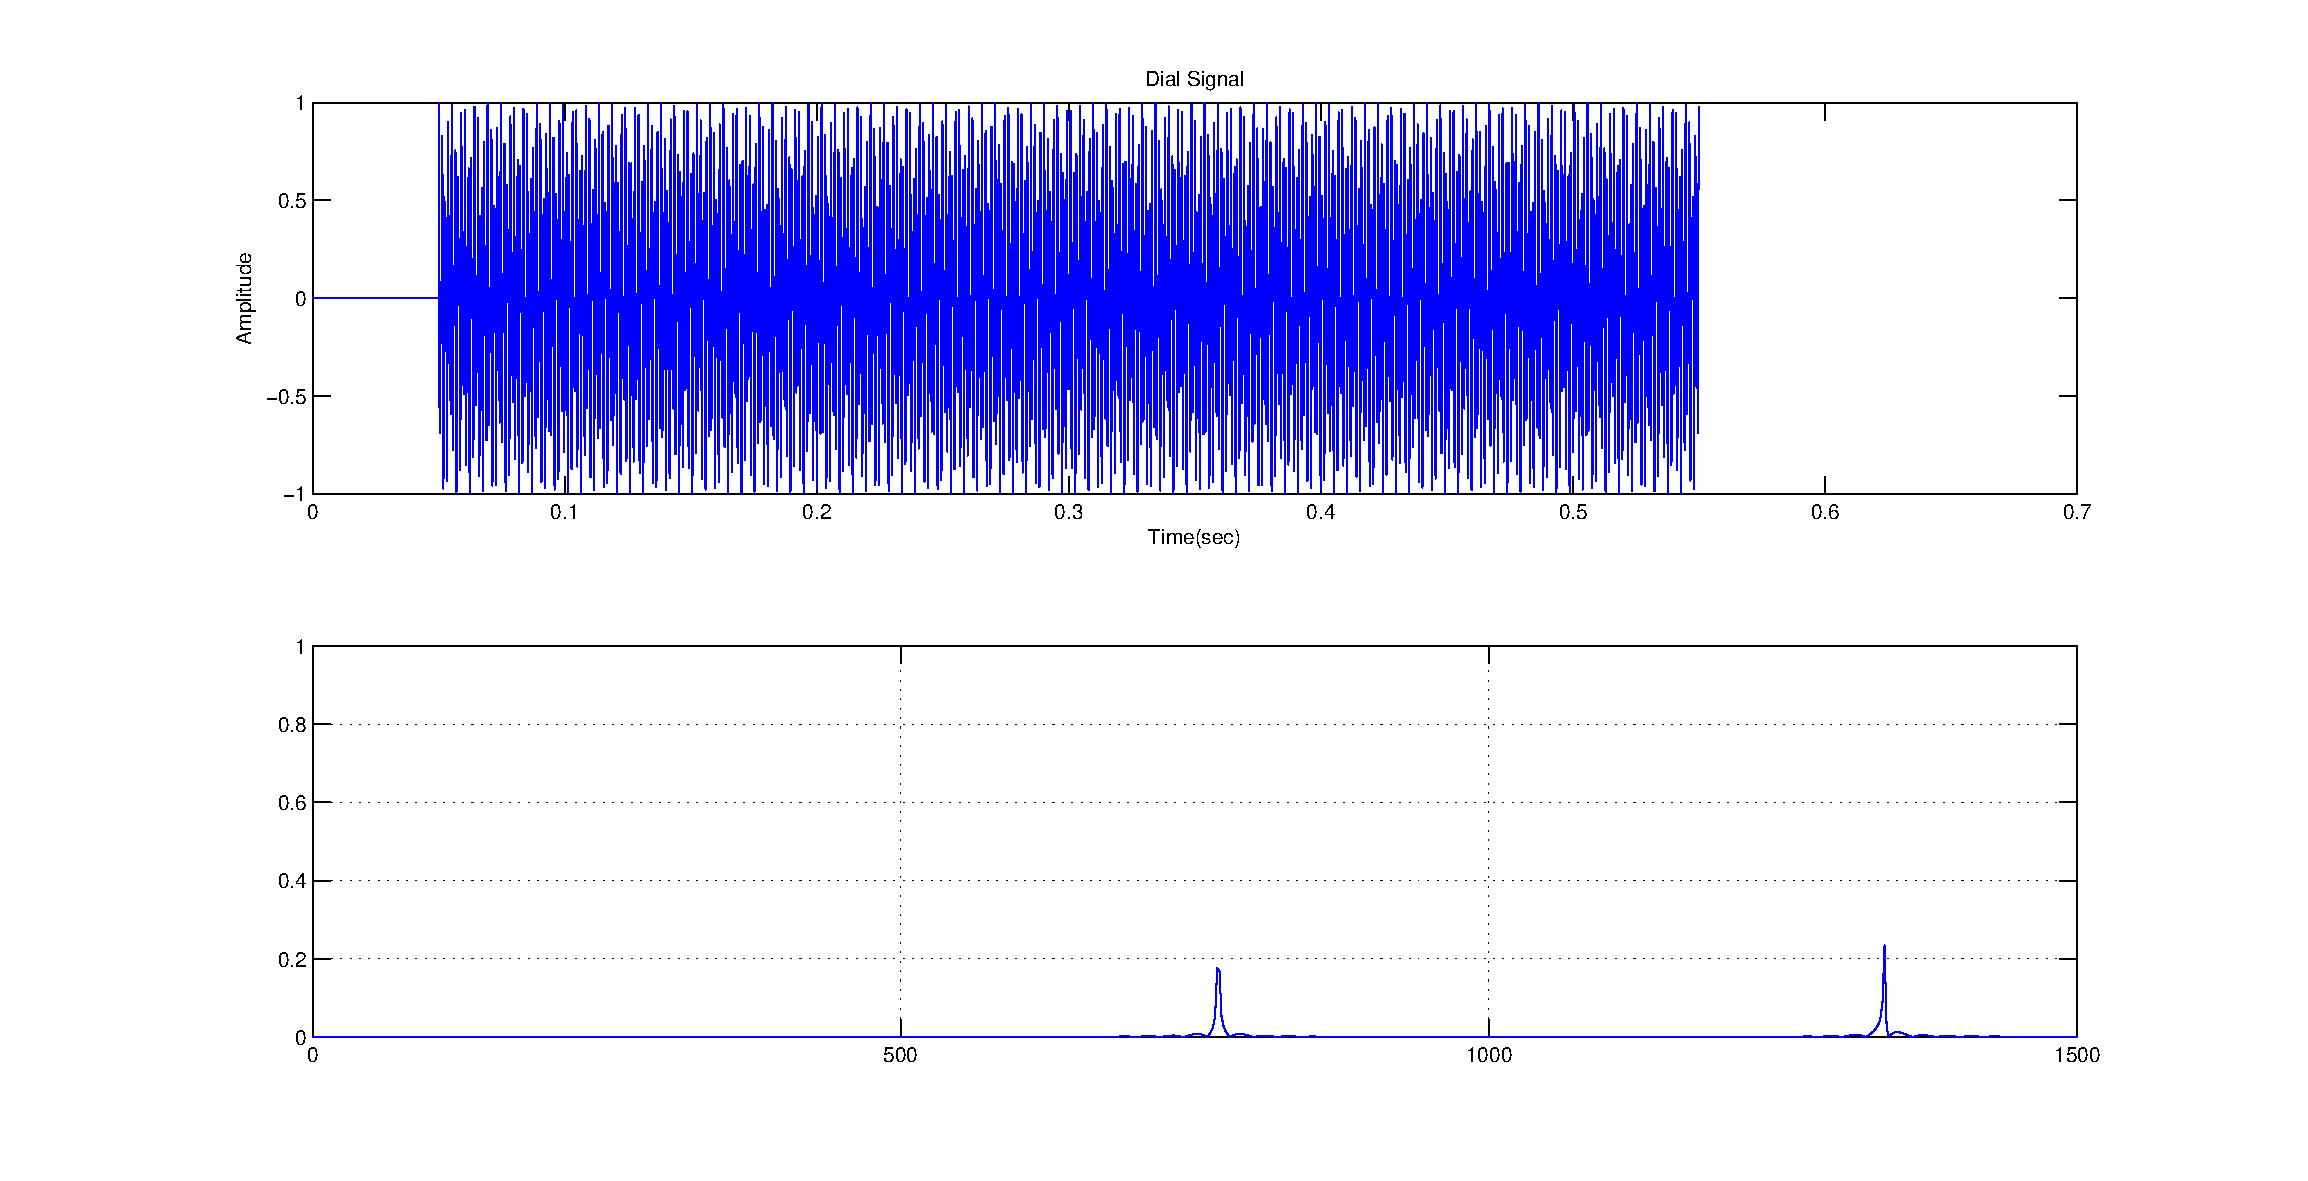
\includegraphics[width=\textwidth]{img43421}
                \caption{\texttt{dial\_tones} mit Eingabe \texttt{5}}
            \end{figure}
            \begin{figure}[H]
                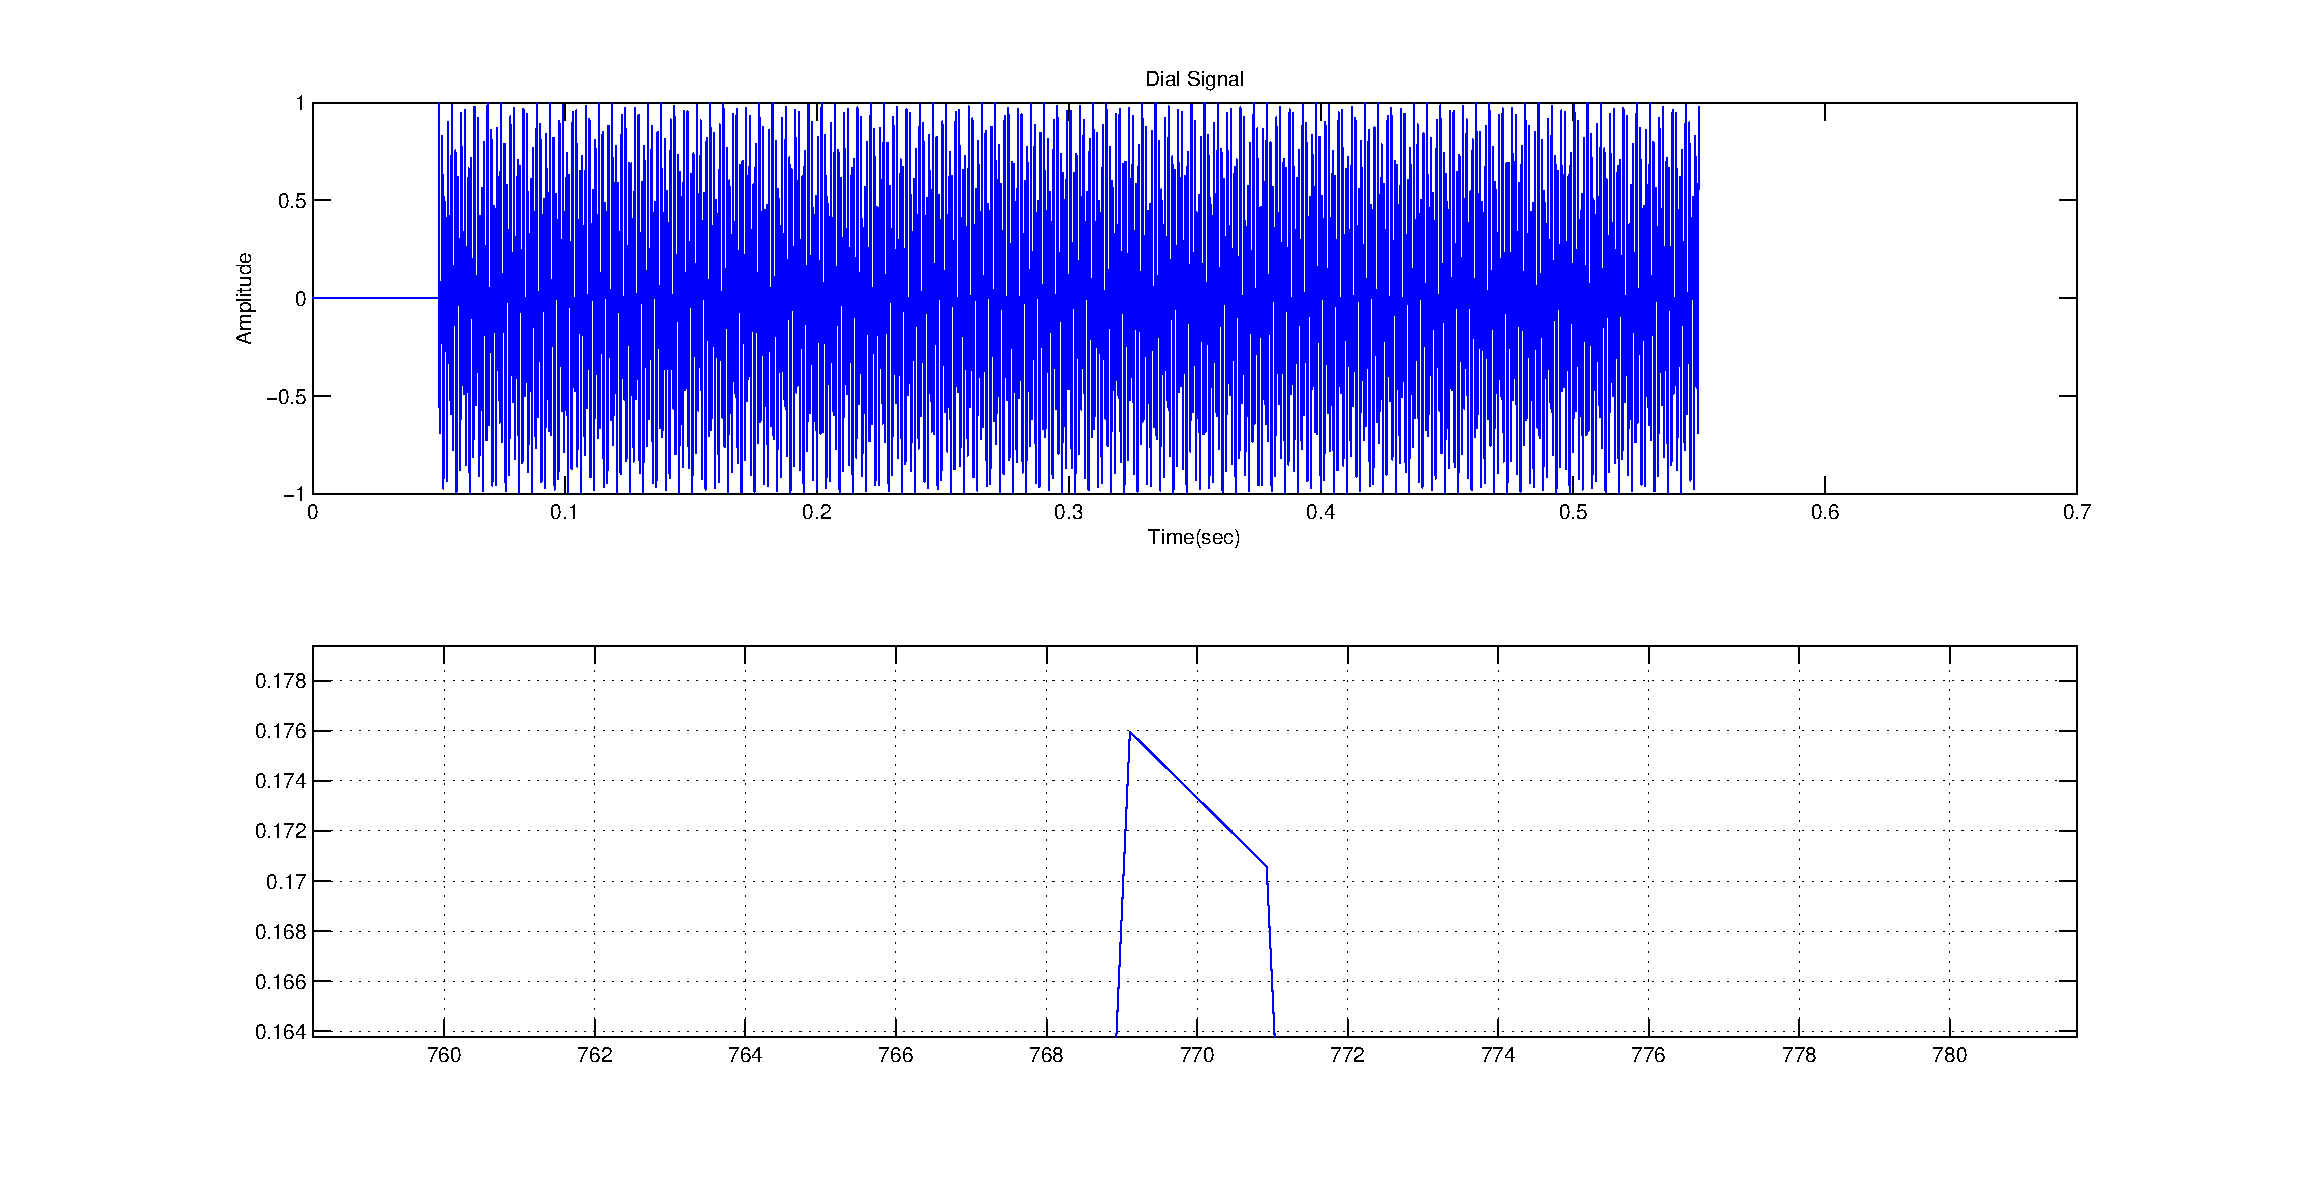
\includegraphics[width=\textwidth]{img43421detail}
                \caption{\texttt{dial\_tones} mit Eingabe \texttt{5}, Zoom bei 770Hz}
            \end{figure}
            \begin{figure}[H]
                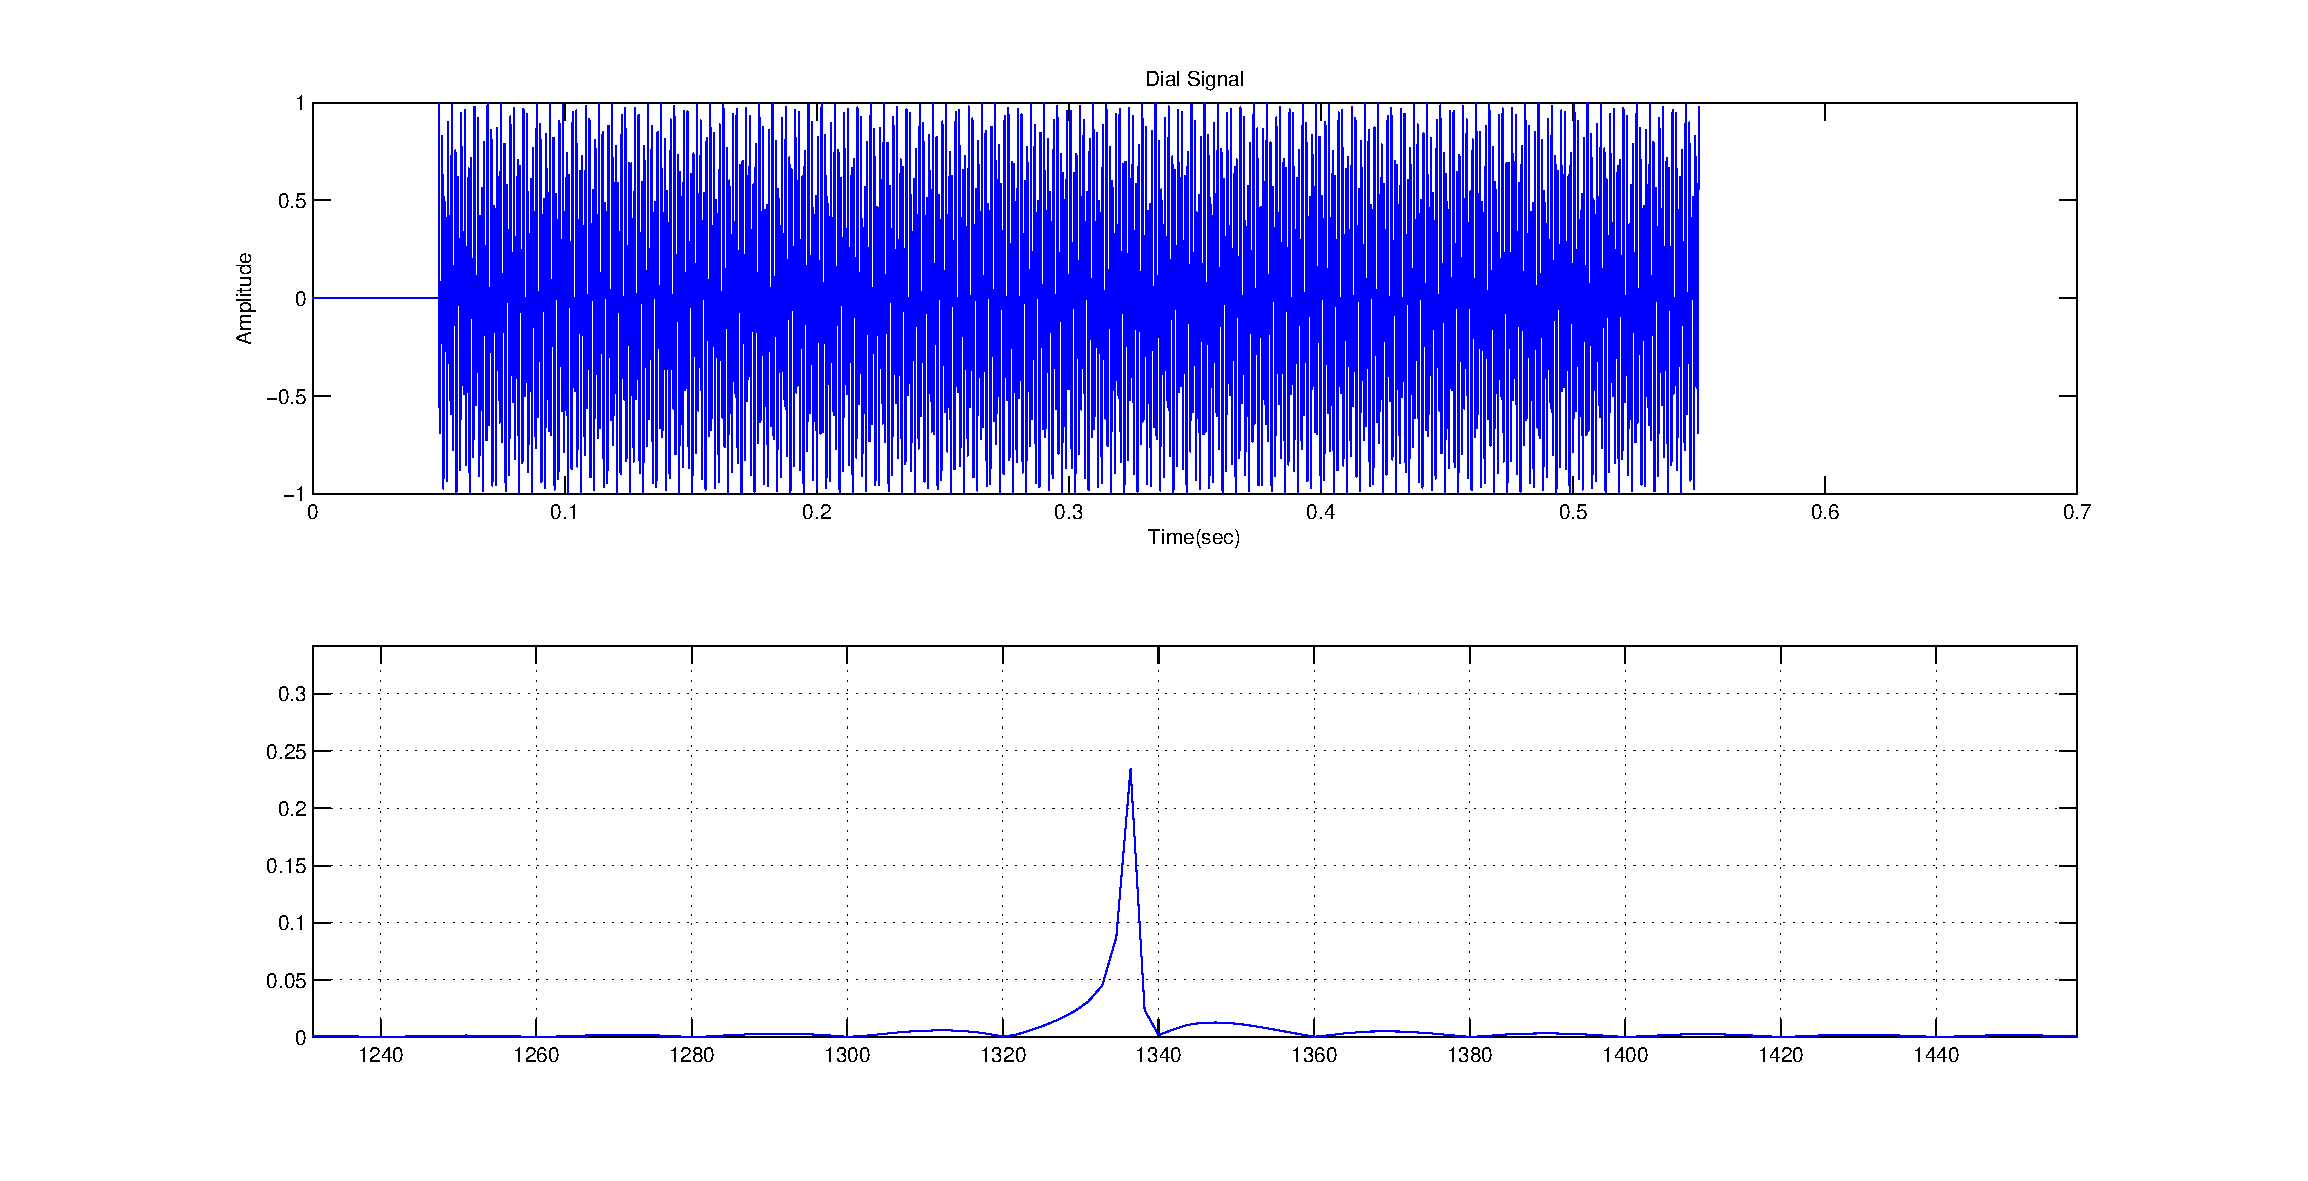
\includegraphics[width=\textwidth]{img43421detail2}
                \caption{\texttt{dial\_tones} mit Eingabe \texttt{5}, Zoom bei 1330Hz}
            \end{figure}
        \end{center}
        Im Frequenzbereich sind die beiden Peaks vergleichsweise breit. Das heißt die
        Frequenzbestimmung ist ungenauer. Trotzdem ist die gedrückte Taste immer
        noch einwandfrei bestimmbar, da der Peak immer noch sehr nah an der
        gewünschten Frequenz liegt und die verschiedenen Frequenzen sehr große
        Abstände haben.

        \vspace{2cm}

        \begin{center}
            \begin{figure}[H]
                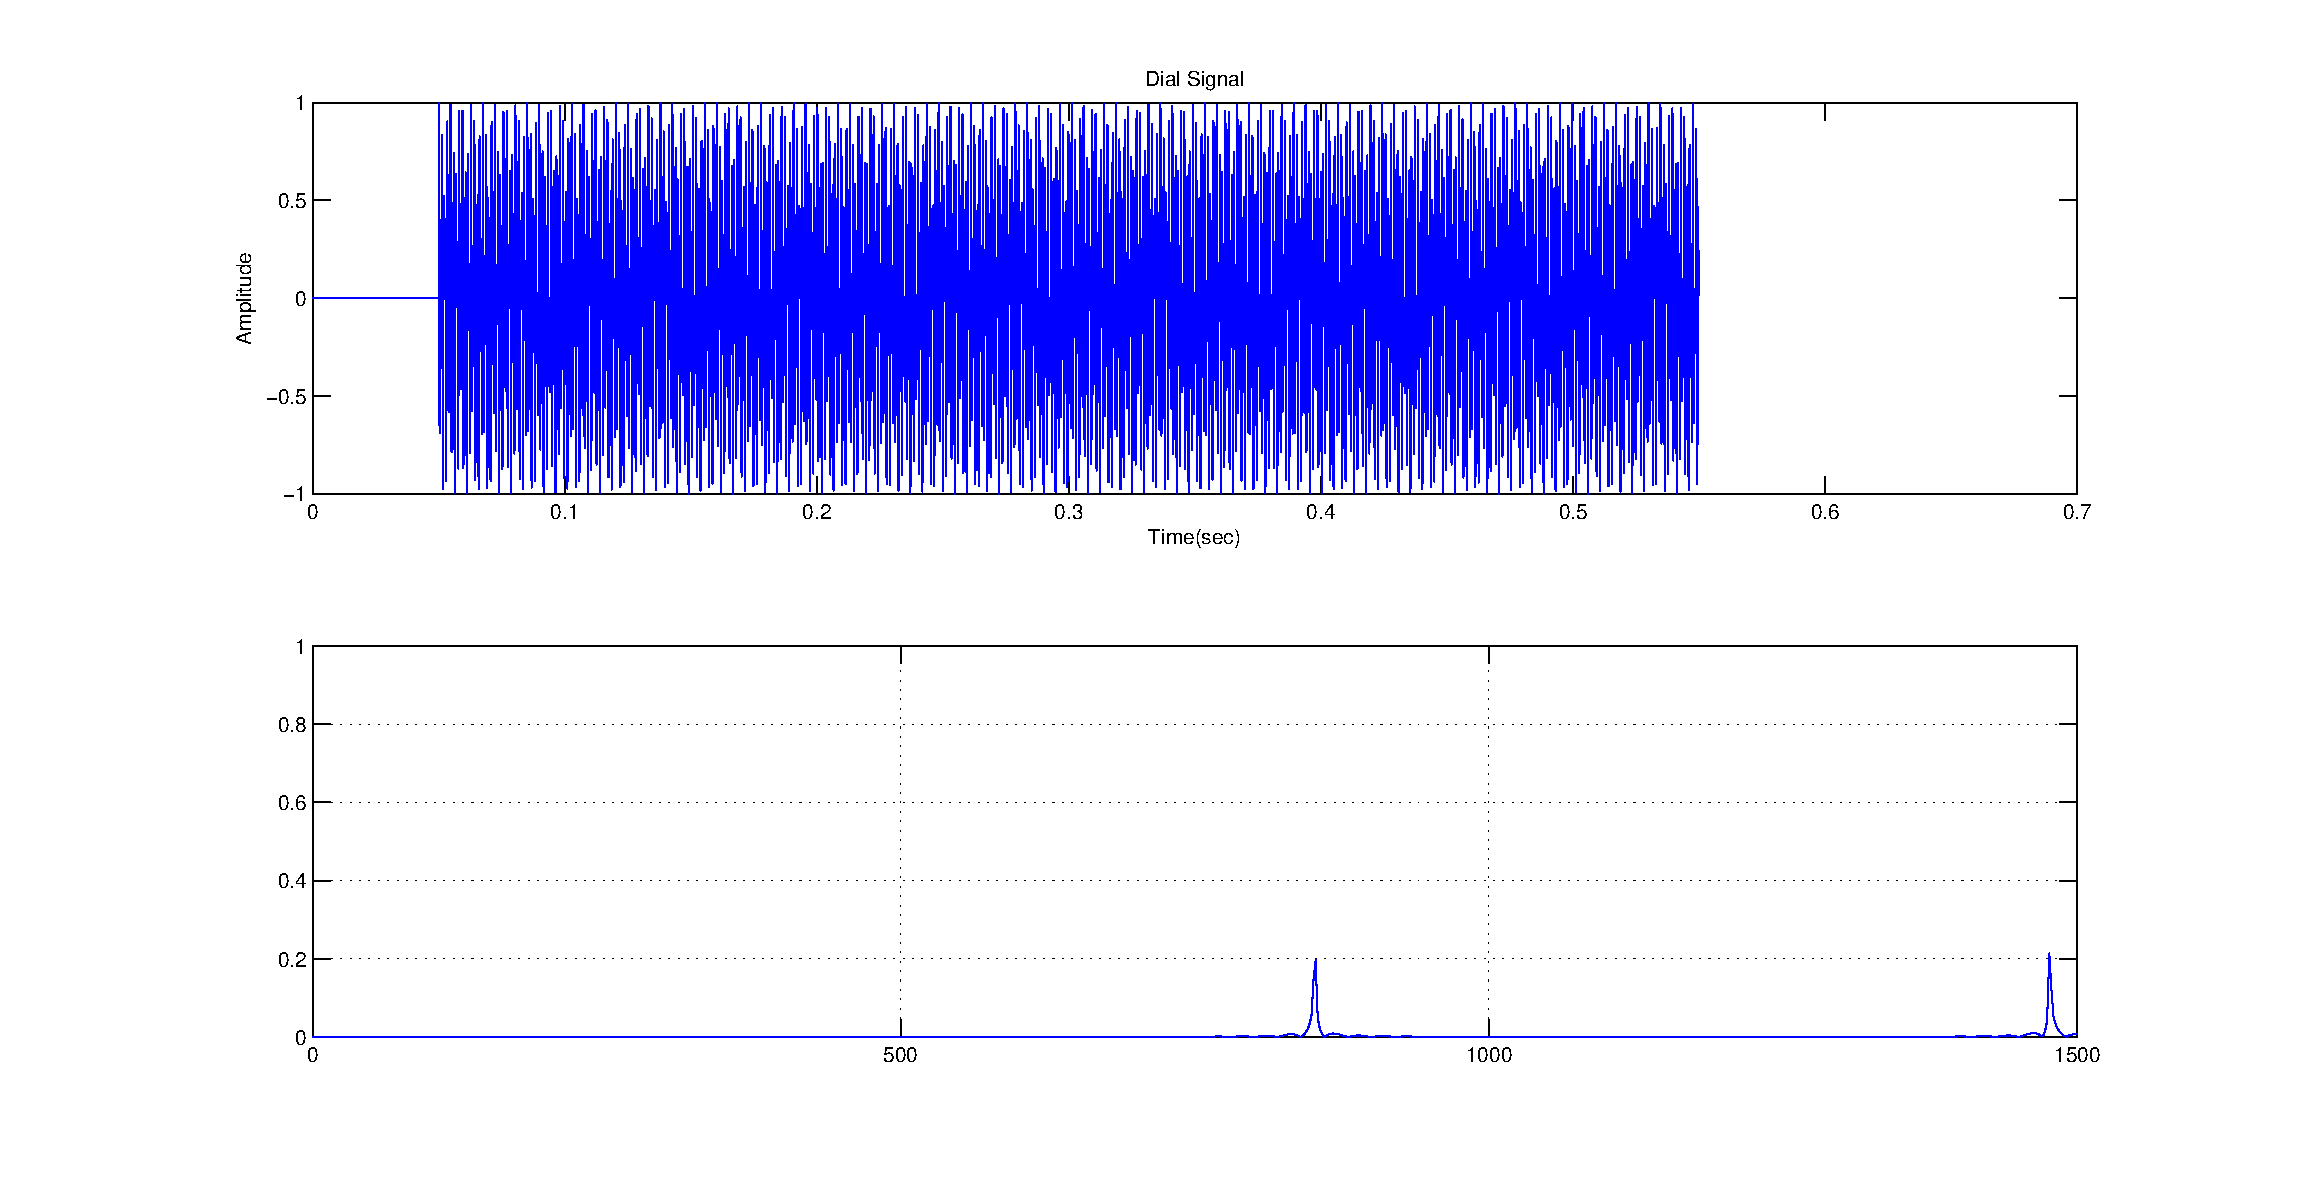
\includegraphics[width=\textwidth]{img43422}
                \caption{\texttt{dial\_tones} mit Eingabe \texttt{9}}
            \end{figure}
        \end{center}

        \subsection{Identifikation einer unbekannten Nummer}
        \paragraph{Einführung}
        Das in der Datei \texttt{dialed\_number.mat} gespeicherte Signal enthält das DTMF-Signal einer
        12-stelligen Telefonnummer.


        \subsubsection{Import}
        \paragraph{Aufgabe}
        Importieren Sie das Signal in MATLAB und hören Sie es sich mit Hilfe der Funktion
        \texttt{soundsc} an. Zusätzlich zur Variablen \glqq{}number\grqq{} muss für \texttt{soundsc} die Abtastrate
        von 32 768 Hz übergeben werden.

        \subsubsection{Code vervollständigen}
        \paragraph{Aufgabe}
        Die Funktion \texttt{fft\_dtmf.m} enthält einige Fragmente die vervollständigt werden sollen
        um das gesamte DTMF Signal in Zeit- und Frequenzbereich plotten zu können. Vervollständigen Sie den Code. Hinweis: eine solche Funktion ist bereits in
        \texttt{dial\_tones}
        implementiert, es müssen lediglich die entsprechenden Zeilen kopiert werden.
        \paragraph{Protokoll}

        \lstinputlisting[language=Matlab]{fft_dtmf_Student.m}

        \subsubsection{Identifikation der Nummer mittels FFT}
        \paragraph{Aufgabe}
        Ist es möglich mittels der Fourier Transformation über das gesamte Signal die
        gewählte Nummer zu identifizieren? Falls nein, wie muss statt dessen vorgegangen werden?

        \paragraph{Protokoll}
        Da im Frequenzbereich nicht sichtbar ist welche Frequenzen zu welcher Zeit
        im Signal vorhanden war lassen sich die Nummern nicht aus dem gesamten
        Signal rekonstruieren.

        Das Signal muss zwischen den Tönen getrennt werden und die Segmente müssen
        einzeln untersucht werden. Dann sind pro Segment nur zwei Peaks im
        Frequenzbereich aus denen sich dann die gedrückte Taste rekonstruieren
        lässt.

        \subsubsection{Plot}
        \paragraph{Aufgabe}
        Ermitteln Sie nun unter Verwendung von \texttt{receive\_dial} die Fourier Transformierte
        über die einzelnen Zeitabschnitte. Fügen Sie einen Plot von drei der auftretenden
        Ziffern im Frequenzbereich in das Protokoll ein und geben Sie die Frequenzen sowie
        die gewählten Ziffern an.

        \paragraph{Protokoll}
        \begin{center}
            \begin{figure}[H]
                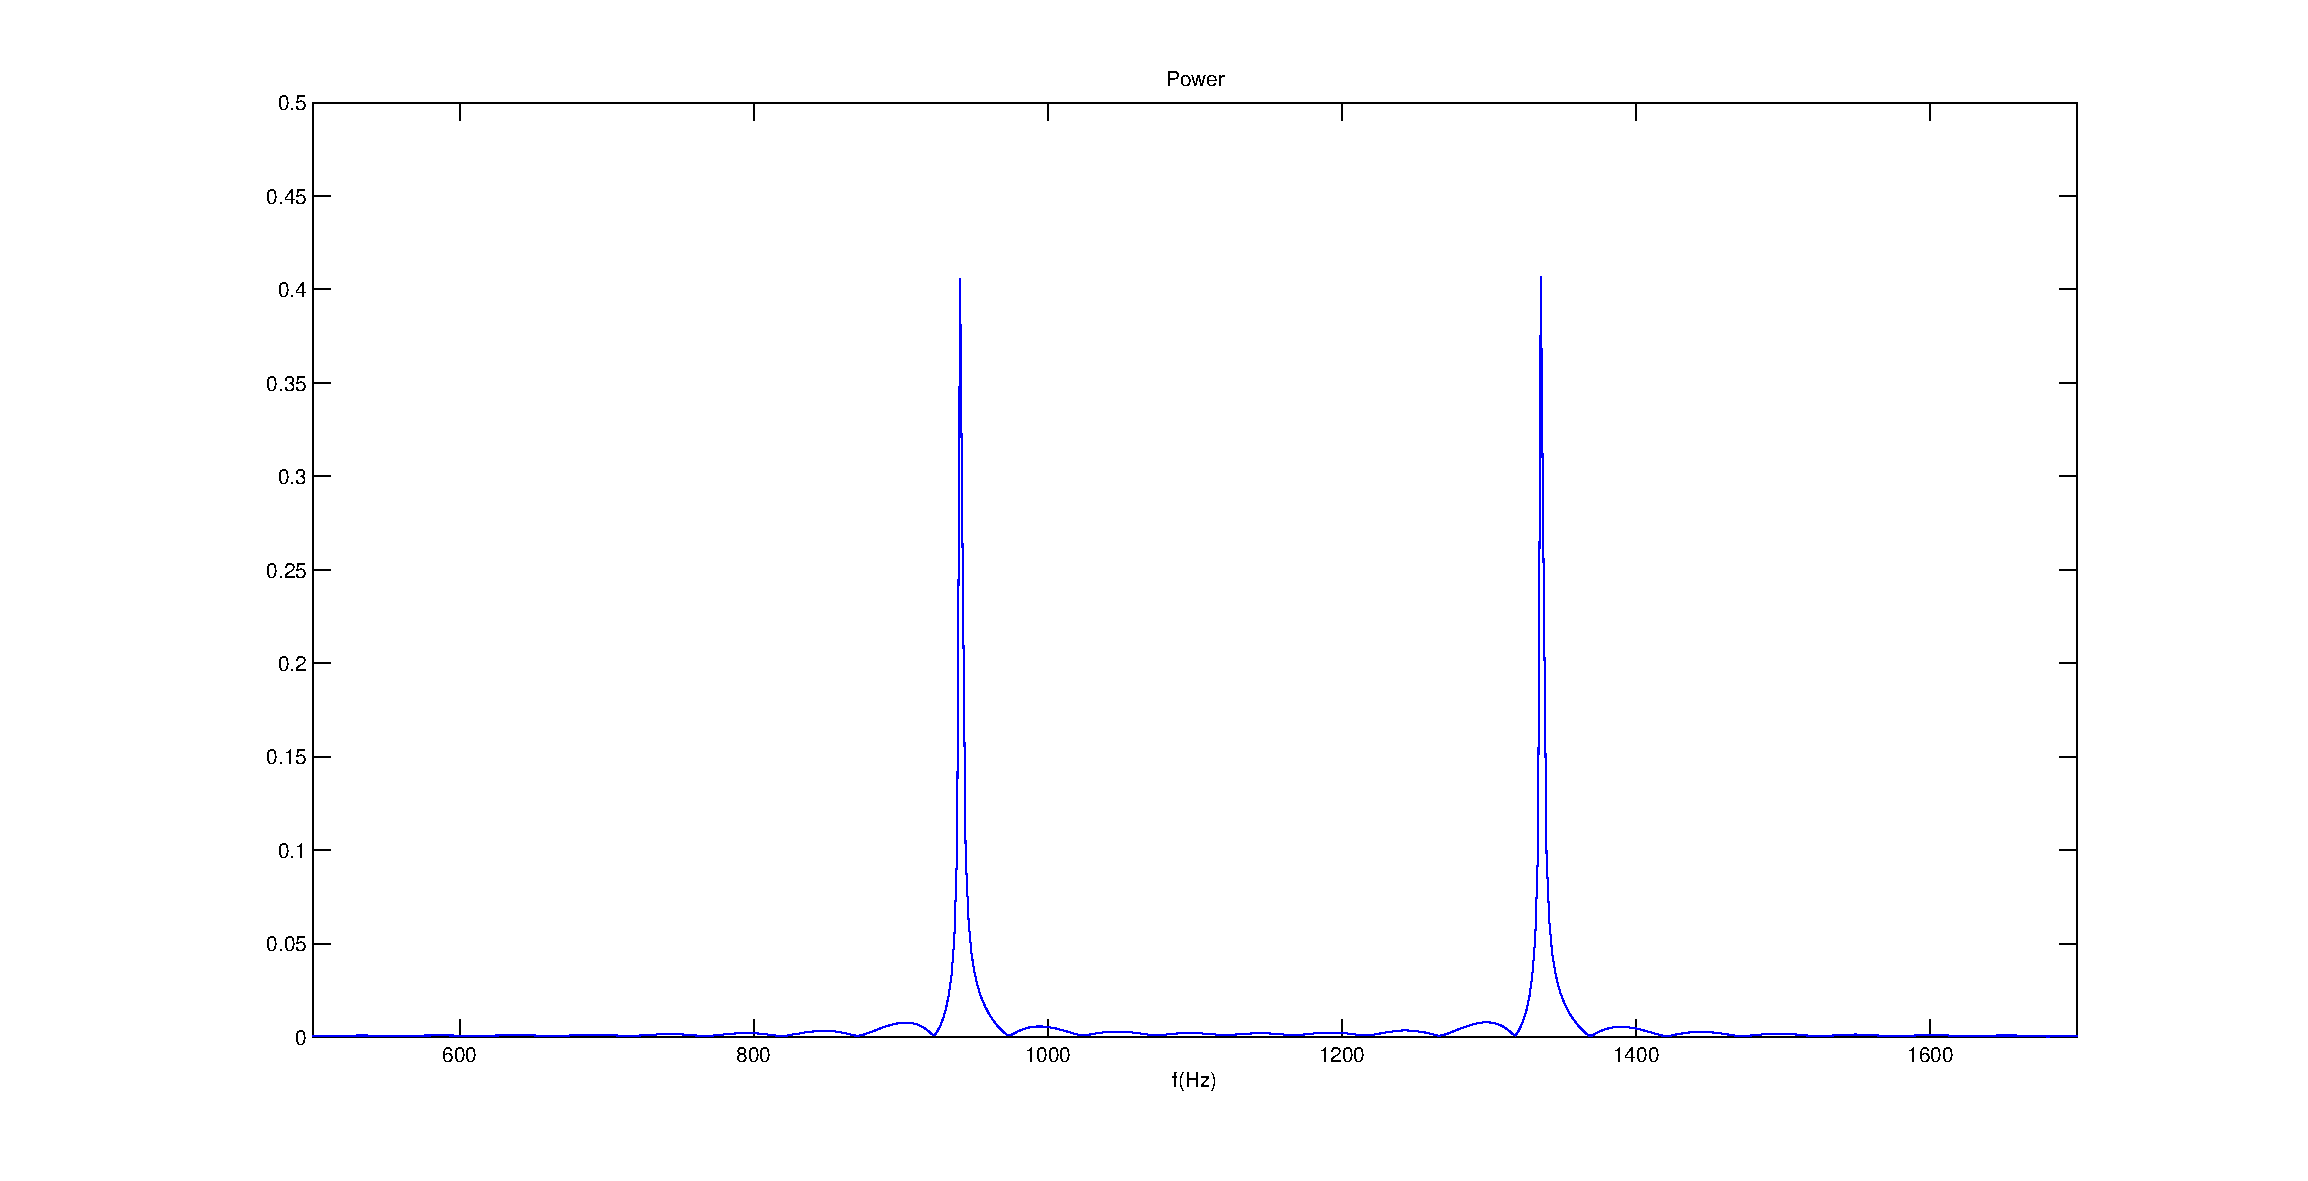
\includegraphics[width=\textwidth]{img43541}
                \caption{Erster Ton mit \texttt{receive\_dial}}
            \end{figure}
        \end{center}
        \begin{eqnarray*}
            f_1 &=& 941 \si{\hertz}\\
            f_2 &=& 1336 \si{\hertz}\\
            &\Rightarrow& \text{Taste: }0
        \end{eqnarray*}

        \begin{center}
            \begin{figure}[H]
                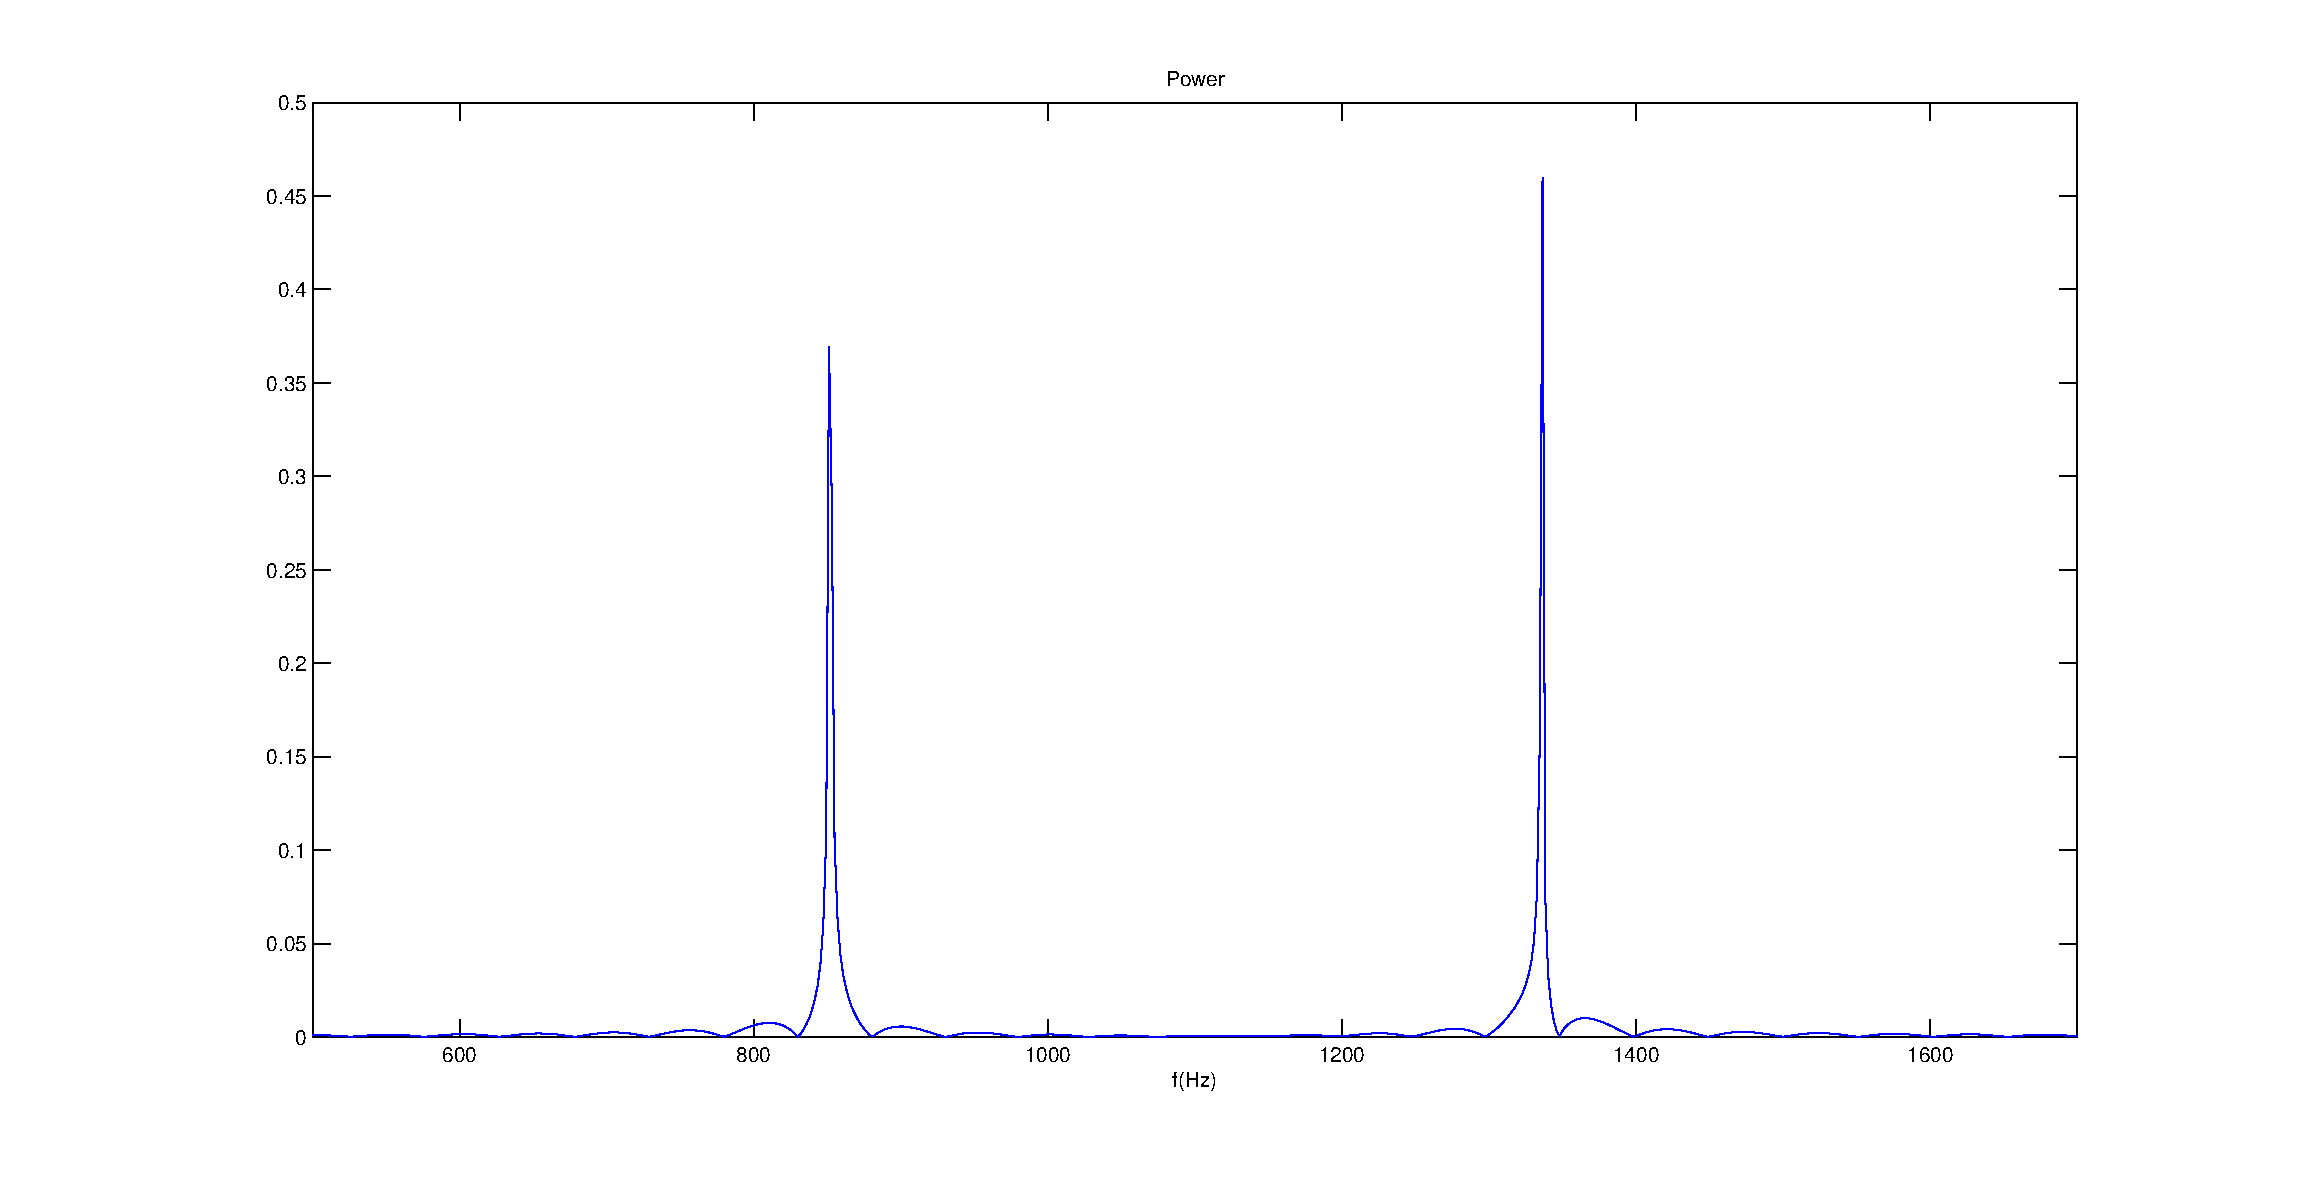
\includegraphics[width=\textwidth]{img43542}
                \caption{Zweiter Ton mit \texttt{receive\_dial}}
            \end{figure}
        \end{center}
        \begin{eqnarray*}
            f_1 &=& 852 \si{\hertz}\\
            f_2 &=& 1336 \si{\hertz}\\
            &\Rightarrow& \text{Taste: }8
        \end{eqnarray*}

        \begin{center}
            \begin{figure}[H]
                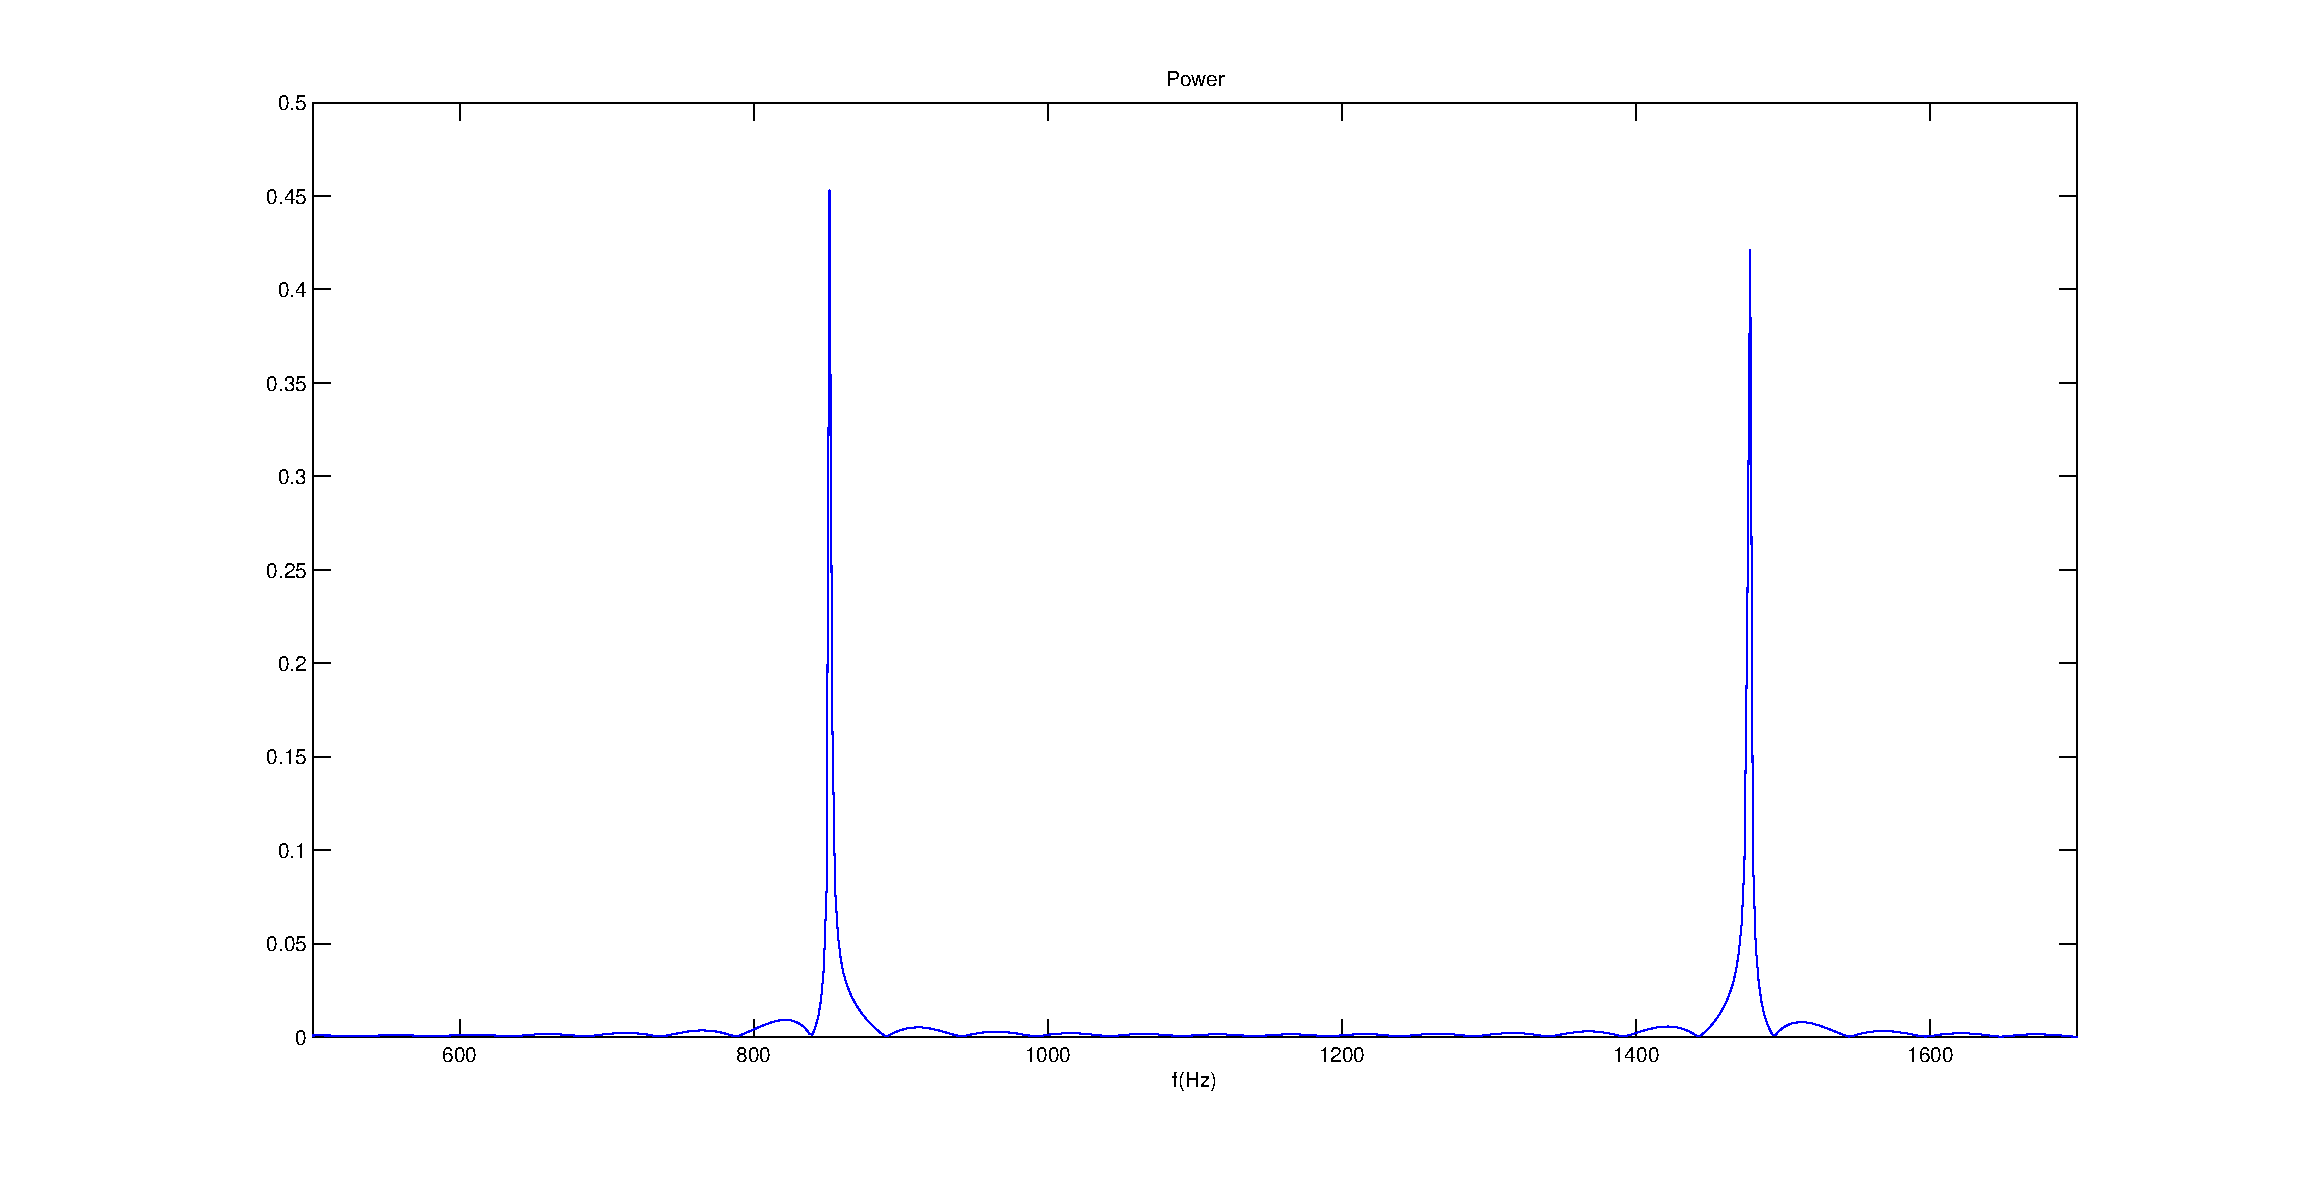
\includegraphics[width=\textwidth]{img43543}
                \caption{Dritter Ton mit \texttt{receive\_dial}}
            \end{figure}
        \end{center}
        \begin{eqnarray*}
            f_1 &=& 852 \si{\hertz}\\
            f_2 &=& 1477 \si{\hertz}\\
            &\Rightarrow& \text{Taste: }9
        \end{eqnarray*}


        \subsubsection{Telefonnummer}
        \paragraph{Aufgabe}
        Wie lautet die gewählte Telefonnummer?

        \paragraph{Protokoll}
        Die Frequenzen wurden jeweils dem Diagramm im Frequenzbereich entnommen
        und daraus die nächste mögliche Frequenz bestimmt.

        Aus den beiden Frequenzen lässt sich die Taste bestimmen.
        \begin{center}
            \begin{tabular}{ccc}
                \toprule
                $f_1$ & $f_2$ & Taste \\
                \midrule
                941 & 1336 & 0\\
                852 & 1336 & 8\\
                852 & 1477 & 9\\
                770 & 1209 & 4\\
                770 & 1336 & 5\\
                697 & 1336 & 2\\
                697 & 1477 & 3\\
                770 & 1336 & 5\\
                770 & 1477 & 6\\
                852 & 1209 & 7\\
                941 & 1336 & 0\\
                941 & 1336 & 0\\
                \bottomrule
            \end{tabular}
        \end{center}
        Die Nummer lautet:
        \begin{equation*}
            089452356700
        \end{equation*}



        \subsubsection{Code}
        \paragraph{Aufgabe}
        In der Funktion \texttt{receive\_dial} wird das Ergebnis der Fourier Transformierten der
        einzelnen Zeitabschnitte berechnet. In welcher Code Zeile geschieht dies?

        \paragraph{Protokoll}
        Die Fourier-Transformation wird jeweils in Zeile 16 berechnet:
        \lstinputlisting[language=Matlab, firstline=16, lastline=16]{receive_dial.m}


        \subsubsection{Code}
        \paragraph{Aufgabe}
        Wie wird anschließend entschieden um welche Nummer es sich handelt?

        \paragraph{Protokoll}
        Zuerst wird im Frequenzbereich versucht die Peaks zu identifizieren,
        dann wird für jeden Peak versucht der Wert einer Taste
        zuzuordnen, dafür muss die Abweichung von gemessener Frequenz zu
        \glqq{}Tastenfrequenz\grqq{} kleiner $2\%$ sein. Aus der Frequenz der Spalte
        und Reihe kann dann die Taste bestimmt werden.
        \lstinputlisting[language=Matlab, firstline=25, lastline=50]{receive_dial.m}

\end{document}
